\begin{section}{Complex Algebra}
	\begin{subsection}{Polar coordinates}
		$$(r,\theta) $$

	\end{subsection}
	\begin{subsection}{Basic identiies and formulas}
		Basic convertions:
		$$y = r ( \sin (\theta) ) $$
		$$x = r ( \cos (\theta) ) $$
		$$r = \sqrt{x^2 + y^2} $$
		$$\theta = \tan^{-1} (\frac{x}{y} ) $$

		Basic Formulas:
		$$-i  = \frac{1}{i} $$
		$$Z = a + bi$$
		$$\overline{Z} = a - bi $$
		$$ \overline{Z} + \overline{w} = \overline{Z + w}$$
		$$\overline{Z} \times Z = \vert Z \vert^2 $$

	
	\end{subsection}
	\begin{subsection}{Euler identity}
		$$e^{iz} = \cos (z) + i \sen (z) $$
		$$e^{\pi i } +1 = 0 $$
	\end{subsection}

	\begin{subsection}{Multiplicative cycles}
		$$i = i$$
		$$i^2 = -1$$
		$$i^3 = -i$$
		$$i^4 = 1$$
		$$i^5 = i$$

	\end{subsection}
	\begin{subsection}{Graphs}
		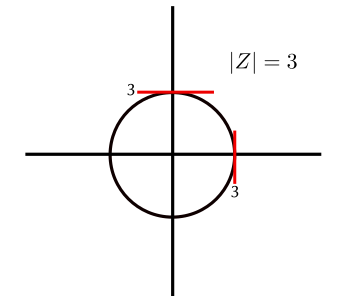
\includegraphics[]{1.png}
	\end{subsection}
	\newpage
	\begin{subsection}{Triangle inequality}
		$$\vert z + w \vert \leq \vert z \vert + \vert w \vert$$
		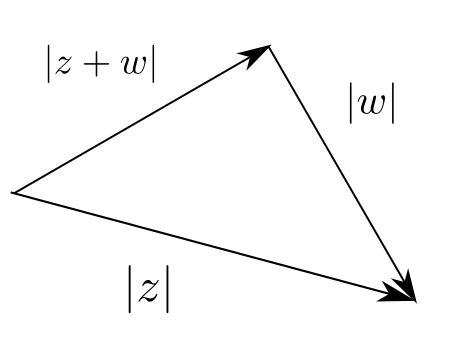
\includegraphics[]{2.png}
	\end{subsection}
	\begin{subsection}{Golden Triangle}
		$$ \frac{a}{b} = \frac{b}{a-b} $$
	\end{subsection}

\end{section}


